\documentclass[tikz,border=2bp]{standalone}
\usepackage{ctex}
\usetikzlibrary{arrows.meta}
\begin{document}
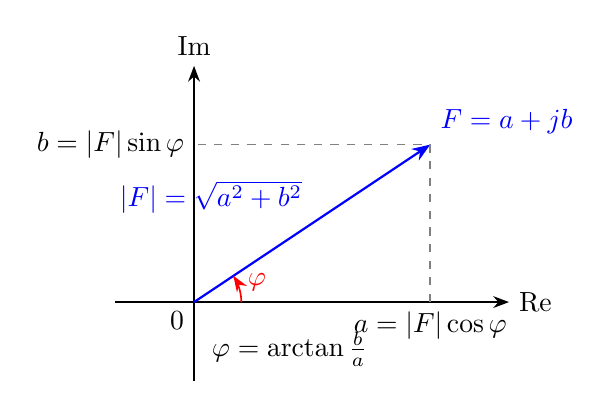
\begin{tikzpicture}[>=Stealth, semithick]
    \draw[->] (-1,0) -- (4,0) node[right] {Re};
    \draw[->] (0,-1) -- (0,3) node[above] {Im};
    \draw[->, thick, blue] (0,0) -- (3,2) node[above right] {$F = a + jb$};
    \draw[dashed, gray] (3,0) -- (3,2) -- (0,2);
    \node[below] at (3,0) {$a = |F|\cos\varphi$};
    \node[left] at (0,2) {$b = |F|\sin\varphi$};
    \node[below left] at (0,0) {$0$};
    \draw[domain=0:33.69,->,red] plot ({0.6*cos(\x)}, {0.6*sin(\x)});
    \node[red] at (0.8,0.25) {$\varphi$};
    \node[blue, above left] at (1.5,1) {$|F| = \sqrt{a^2+b^2}$};
    \node[right, align=left] at (0.1,-0.6) {$\varphi = \arctan \frac{b}{a}$};
\end{tikzpicture}

\begin{tikzpicture}[>=Stealth, semithick]
    \draw[->] (-2.5,0) -- (2.5,0) node[right] {Re};
    \draw[->] (0,-2.5) -- (0,2.5) node[above] {Im};
    \node[red, font=\small] at (1.5,1.5) {I象限: $\varphi = \theta$};
    \node[red, font=\small] at (-1.5,1.5) {II象限: $\varphi = \theta + 180^\circ$};
    \node[red, font=\small] at (-1.5,-1.5) {III象限: $\varphi = \theta - 180^\circ$};
    \node[red, font=\small] at (1.5,-1.5) {IV象限: $\varphi = \theta$};
    \node[gray, font=\scriptsize] at (1.5,1.1) {($a>0, b>0$)};
    \node[gray, font=\scriptsize] at (-1.5,1.1) {($a<0, b>0$)};
    \node[gray, font=\scriptsize] at (-1.5,-1.1) {($a<0, b<0$)};
    \node[gray, font=\scriptsize] at (1.5,-1.1) {($a>0, b<0$)};
    \node[below right, align=left] at (-2.4,-1.8) {注: $\theta = \arctan \frac{b}{a}$ 为计算器计算值};
\end{tikzpicture}
\end{document}
